\documentclass{standalone}
\usepackage{tikz}
\usepackage{bm}
\usetikzlibrary{fit,positioning}
\begin{document}
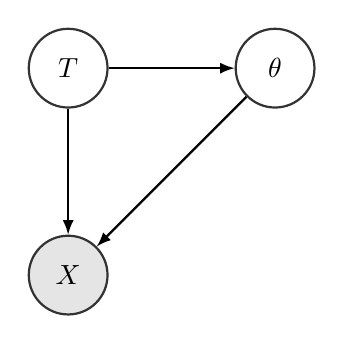
\begin{tikzpicture}
\tikzstyle{main}=[circle, minimum size = 10mm, thick, draw =black!80, node distance = 16mm]
\tikzstyle{connect}=[-latex, thick]
\tikzstyle{box}=[rectangle, draw=black!100]
  \node[main] (c) [] { $T$ };
  \node[main] (theta) [right=of c] { $\theta$ };
  \node[main, fill = black!10] (x) [below=of c] { $X$ };
  \path (c) edge [connect] (x)
        (c) edge [connect] (theta)
        (theta) edge [connect] (x);
  %\node[rectangle, inner sep=0mm, fit= (x),label=below right:N, xshift=-1mm, yshift=1mm] {};
  %\node[rectangle, inner sep=4.4mm,draw=black!100, fit= (x)] {};
  %\node[rectangle, inner sep=4.6mm, fit= (z) (f),label=below right:N, xshift=-1mm, yshift=-12mm] {};
  %\node[rectangle, inner sep=9mm, draw=black!100, fit = (z) (f)] {};
\end{tikzpicture}
\end{document}
